\subsection*{Results}

\begin{figure*}
    \vspace{3cm}
    \rlap{
        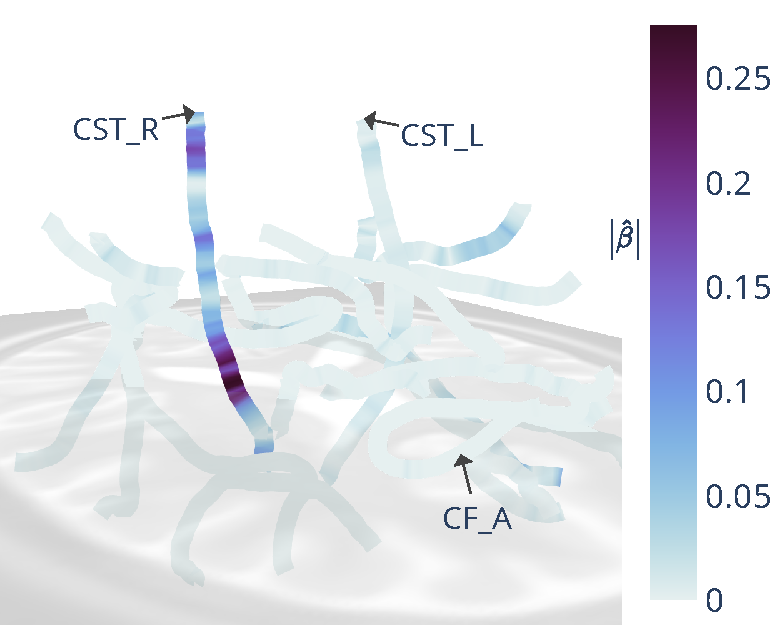
\includegraphics[width=0.33\textwidth]{als_coefs.pdf}
    }
    \vspace{-8.4cm}
    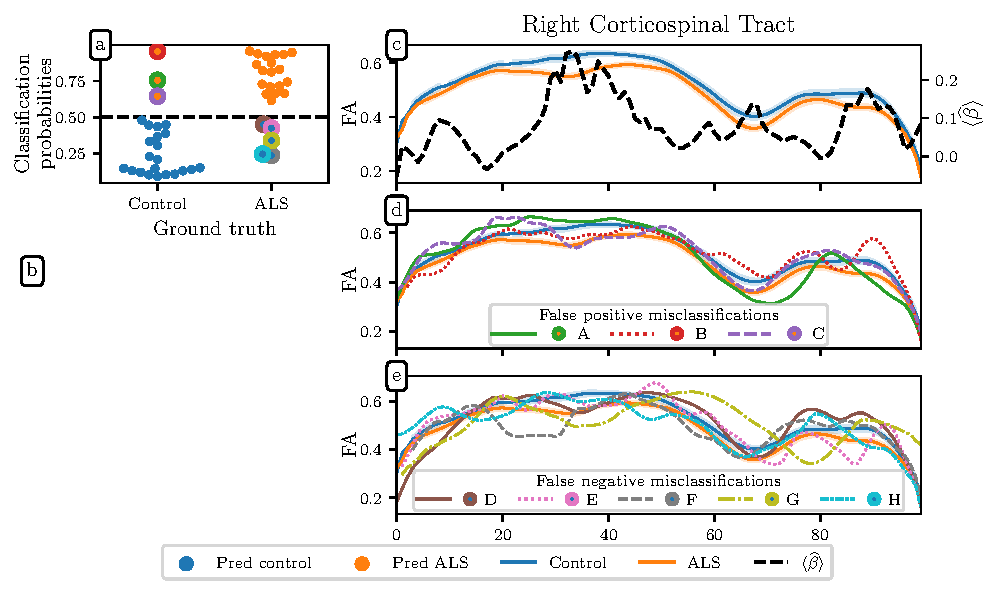
\includegraphics[width=\textwidth]{als_results.pdf}
    {\phantomsubcaption\label{fig:class-results:probs}}
    {\phantomsubcaption\label{fig:class-results:coefs3d}}
    {\phantomsubcaption\label{fig:class-results:tract-profiles}}
    {\phantomsubcaption\label{fig:class-results:false-positives}}
    {\phantomsubcaption\label{fig:class-results:false-negatives}}
    \caption{%
        {\bf SGL accurately and interpretably predicts ALS diagnosis.}
        \label{fig:class-results}
        {\bf (a)} Classification probabilities for ALS diagnosis, with
        controls on the left, patients on the right, predicted controls in
        blue, and predicted patients in orange. So orange dots on the left
        represent false positives, while blue dots on the right represent
        false negatives. We achieve {\protect\alsAccuracy}\% accuracy with an
        ROC AUC of {\protect\alsRocAuc}.
        {\bf (b)} SGL coefficients are presented on the core fibers of major
        fiber bundles. They exhibit high group sparsity and are concentrated
        in the fa of the CST. The brain is oriented with the right hemisphere
        in the foreground and anterior to the right of the page. The CST\_L,
        CST\_R, and CF\_A bundles are indicated for orientation.
        {\bf (c)} SGL identifies three portions of the CST as important,
        where $\hat{\beta}$ (dashed line, right axis) has large values. These
        are centered around nodes 30, 65, and 90, corresponding to locations
        of substantial differences in FA between the ALS and control groups
        (shaded areas indicates standard error of the mean).
        {\bf (d)} Bundle profiles for false positive classifications. Line
        colors correspond to the marker edge color in the top left plot.
        These individuals have reduced FA in the CST portions which SGL
        identified as important. Their misclassification is coherent with the
        feature importance and the group differences in FA.
        {\bf (e)} Individual bundle profiles for false negative
        classifications. These individuals have bundle profiles which
        oscillate between the group means.
    }
\end{figure*}

We developed a method for analyzing dMRI tractometry data with SGL. We
demonstrate the use of this method on four previously published datasets in
both a classification setting and a regression setting.

\subsubsection*{SGL accurately detects ALS from tractometry data}

Using data from a previous study of the corticospinal tract (CST) profile and
ALS \cite{sarica2017corticospinal}, we tested the performance of SGL in a
classification setting. The previous study predicted ALS status with a mean
accuracy of 80\% using a random forest algorithm based on a priori selection
of features within the corticospinal tract. SGL delivers competitive
predictive performance (mean {\alsAccuracy}\% accuracy, {\alsRocAuc} ROC AUC)
without the need for a priori feature engineering. The results of the
classification prediction are shown in \cref{fig:class-results:probs} with
``ground-truth'' ALS status separated into columns, and predicted ALS status
encoded by color. In addition to this classification performance, SGL also
identifies the white matter tracts most important for ALS classification. The
relative importance of white matter features is captured in the $\beta$
coefficients from \cref{supp:eq:sgl}. \Cref{fig:class-results:tract-profiles}
depicts these coefficients along the right CST, plotted over the FA values
for the control and ALS subject groups. We find that SGL selects FA metrics
in the corticospinal tract and particularly in the right corticospinal tract
as most important to ALS classification, confirming previous findings
\cite{van2011upper, toosy2003diffusion, sarica2014tractography,
sage2007quantitative, sage2009quantitative, karlsborg2004corticospinal,
ellis1999diffusion, cosottini2005diffusion, ciccarelli2009investigation,
abe2010voxel} and identifying the portions of the brain that were selected
\emph{a priori} in the previous study from which we collected our data
\cite{sarica2017corticospinal}.

The $\beta$ coefficients exhibit high bundle level sparsity; only some
bundles are important, which can be be confirmed by observing the value of
$\alpha$ in \cref{supp:eq:sgl}, the regularization hyperparameter that
controls the mixture of the group lasso and lasso penalties. If $\alpha$ is
closer to zero, it indicates that the phenotype in question preferentially
correlates with only a few groups of covariates. For the ALS dataset, $\alpha
= $ \alsLRatio, confirming that the white matter correlates of ALS reside
mostly in one bundle, namely the CST.

Analyzing the ways in which the model mislabels individuals also provides
insight. We found that mislabelled subjects are outliers relative to their
group with respect to diffusion features of the CST.
\Cref{fig:class-results:false-positives,fig:class-results:false-negatives}
depicts the group FA values along with FA values of mislabelled subjects,
four false negatives and three false-positives. The false positive
classifications have reduced FA in one or more of the three sections of the
CST where $\norm*{\hat{\beta}}$ is large
\cref{fig:class-results:tract-profiles}. The false negative subjects have FA
profiles that oscillate between the two group means. Thus, the SGL method
fails comprehensibly.

\begin{figure*}
    \vspace{3.65cm}
    \rlap{
        \hspace{1cm}
        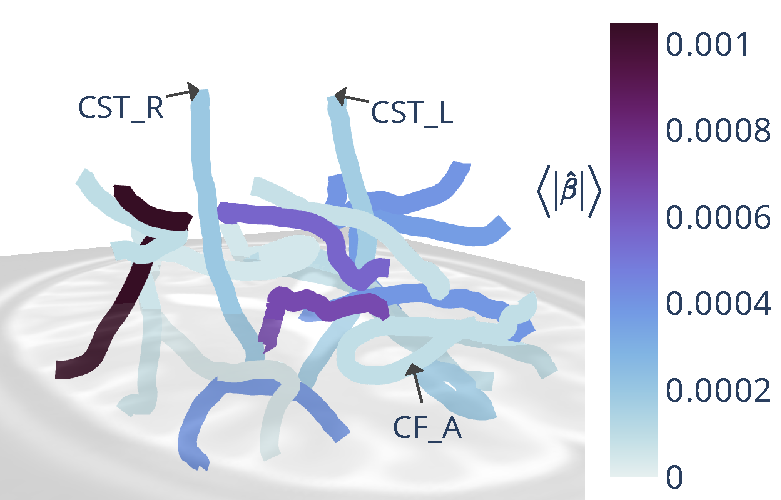
\includegraphics[width=0.275\textwidth]{wh_coefs.pdf}
        \hspace{0.25em}
        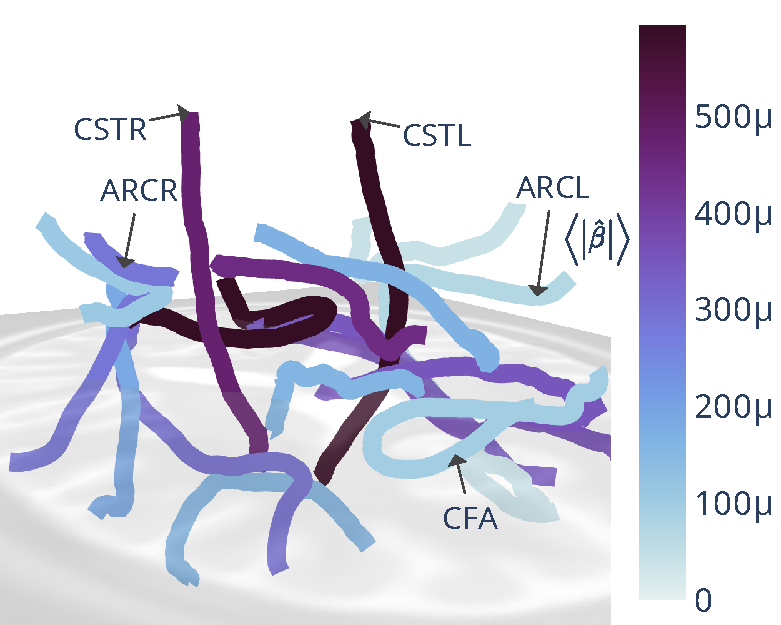
\includegraphics[width=0.275\textwidth]{hbn_coefs.pdf}
        \hspace{0.25em}
        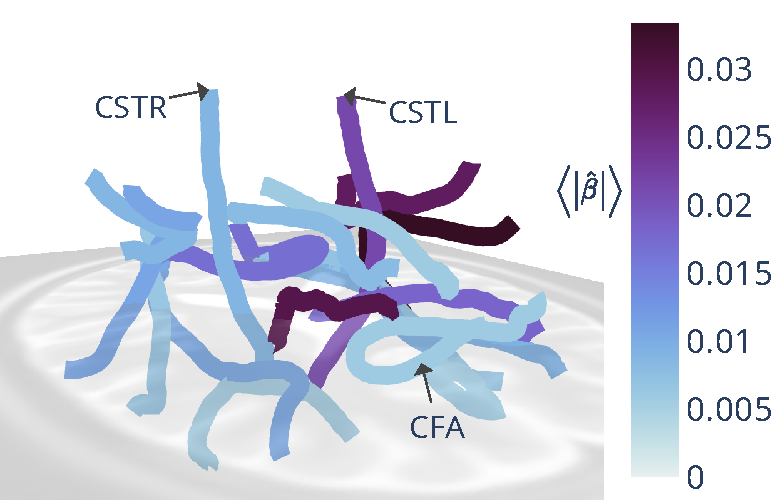
\includegraphics[width=0.275\textwidth]{camcan_coefs.pdf}
    }
    \vspace{-7.3cm}
    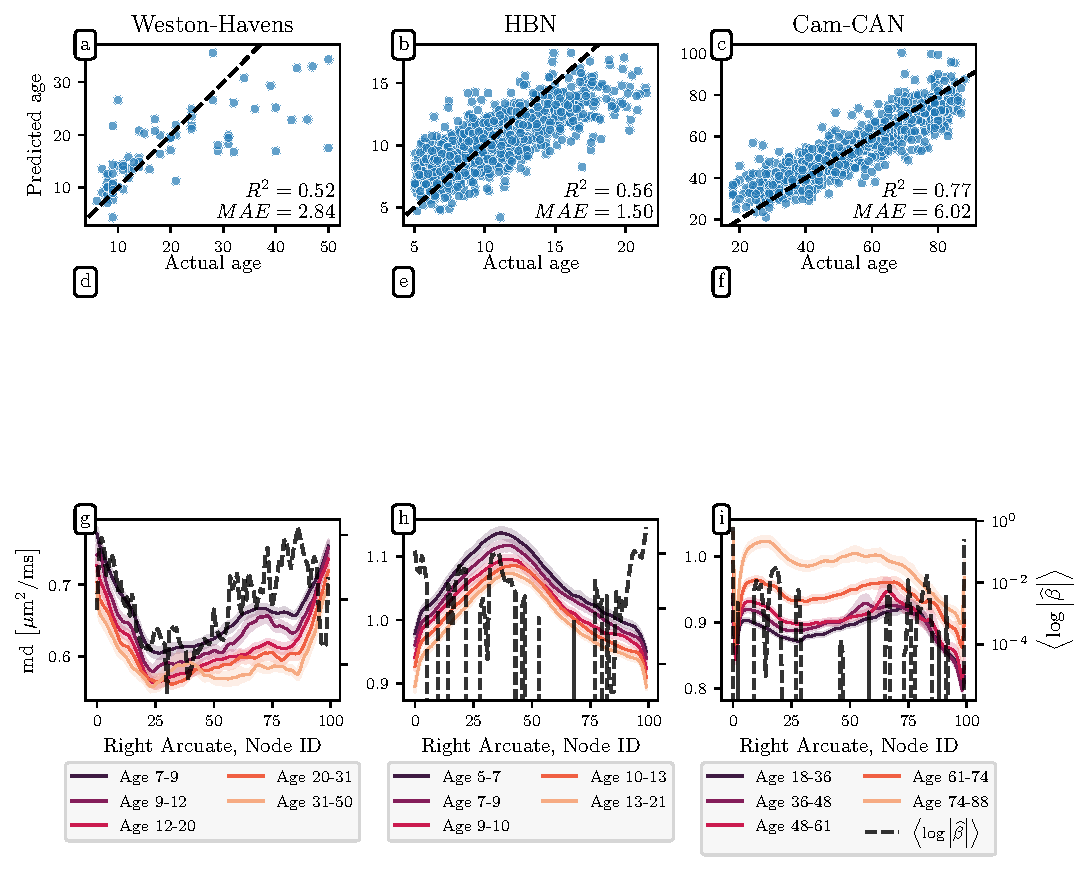
\includegraphics[width=\textwidth]{regression_scatter.pdf}
    {\phantomsubcaption\label{fig:age-results:wh-scatter}}
    {\phantomsubcaption\label{fig:age-results:hbn-scatter}}
    {\phantomsubcaption\label{fig:age-results:cc-scatter}}
    {\phantomsubcaption\label{fig:age-results:wh-coefs3d}}
    {\phantomsubcaption\label{fig:age-results:hbn-coefs3d}}
    {\phantomsubcaption\label{fig:age-results:cc-coefs3d}}
    {\phantomsubcaption\label{fig:age-results:wh-profile}}
    {\phantomsubcaption\label{fig:age-results:hbn-profile}}
    {\phantomsubcaption\label{fig:age-results:cc-profile}}
    \caption{%
        {\bf Predicting age with tractometry and SGL.}
        \label{fig:age-results}
        {\bf (top)} The predicted age vs. true age of each individual from the test
        splits (i.e., when each subject's data was held out in fitting the
        model) for the {\bf (a)} WH, {\bf (b)} HBN, and {\bf (c)} Cam-CAN
        datasets; an accurate prediction falls close to the $y=x$ line
        (dashed). The mean absolute error (MAE) and coefficient of
        determination $R^2$ are presented in the lower right of each scatter
        plot.
        {\bf (middle)} Feature importance for predicting age from tractometry in
        the {\bf (d)} WH, {\bf (e)} HBN, and {\bf (f)} Cam-CAN datasets.
        The orientation of the
        brain is that same as in \cref{fig:class-results:coefs3d}, however because
        the coefficients exhibit high global sparsity (as opposed to group
        sparsity), we plot the mean of the absolute value of $\hat{\beta}$
        for each bundle on the core fiber. The global distrubution of the
        $\hat{\beta}$ coefficients reflects the fact that aging is not
        confined to a single white matter bundle.
        {\bf (bottom)} Age quintile bundle profiles for the {\bf (g)} WH,
        {\bf (h)} HBN, and {\bf (i)} Cam-CAN datasets.
    }
\end{figure*}

\subsubsection*{SGL accurately predicts age from tractometry data}

To test the performance of SGL with tractometry data in a continuous
regression task, we focus here on the prediction of biological age based on
tractometry data in three datasets named WH, HBN, and Cam-CAN (see
\cref{supp:sec:data} for further details). Prediction of ``brain age'' is a
commonly undertaken task in neuroimaging machine learning, in part because
these predictions, and deviations therefrom, may be diagnostic of overall
brain health (for a review, see \textcite{Cole2019-rz}). However, as
\textcite{nelson2019biomarkers} have observed, aging biomarkers are subject
to unique challenges and tend to be noncausative. Our interest in aging here
relies on its utility as a methodological benthmark. Biological age operates
on a natural scale, with meaningful and easily understood units, and it's
popularity as a machine learning target makes it valuable for comparisons
with other studies.

The WH \cite{yeatman2014lifespan}, HBN \cite{alexander2017open}, and Cam-CAN
\cite{shafto2014cambridge,taylor2017cambridge} datasets used here contain
data from 76, 978, and 640 subjects, respectively, ranging from 6-50, 5-21,
and 18-88 years of age, respectively. In each case, biological age was used
as the predicted variable ($y$ in \cref{supp:eq:lm}). SGL was fit to
tractometry-extracted features in 18 major brain tracts: DTI FA and DTI MD
for WH and DKI FA and DKI MD for HBN and Cam-CAN, with each tract divided
into 100 nodes.

To evaluate the fit of the model, we used a nested cross-validation
procedure. In this procedure, batches of subjects are held out. For each
batch (or fold), the model is fully fit without this data. Then, once the
parameters are fixed, the model is inverted to predict the ages of held out
subjects based on the linear coeffiecients. This scheme automatically finds
the right level of regularization (i.e., sparseness) and fits the
coefficients to the ill-posed linear model, while guarding against
overfitting. SGL accurately predicts the age of the subjects in this
procedure, with a median absolute error of 2.8 years, 1.5 years, and 6.0
years for WH, HBN, and Cam-CAN, respectively and coefficients of
determination $R^2 = $ {\whRsq} , {\hbnRsq}, and {\camcanRsq}, respectively (see
\cref{fig:age-results}, top panels). The predictions for Cam-CAN are
competitive with a recent state of the art prediction
\cite{mcpherson2020single}, which used streamline density to estimate the
brain's structural connectivity and achieved $R^2 = 0.63$. The median
absolute errors are also lower than the results of a recent study that
predicted age in a large sample, based on diffusion MRI features
\cite{Richard2018-ux}.

In contrast to the ALS classification case, the selected $\alpha$ values
indicate high global sparsity over group sparsity, with $\alpha = $
{\whLRatio}, {\hbnLRatio}, and {\ccLRatio}, for the WH, HBN, and Cam-CAN
datasets, respectively. The model weights are distributed over many different
tracts and dMRI tissue properties (see
\cref{fig:age-results:wh-coefs3d,fig:age-results:hbn-coefs3d,fig:age-results:cc-coefs3d}
and supplemental material
\cref{supp:fig:wh-bp:md,supp:fig:wh-bp:fa,supp:fig:hbn-bp:md,supp:fig:hbn-bp:fa,supp:fig:cc-bp:md,supp:fig:cc-bp:fa}).
This demonstrates that SGL is not coerced to produce overly sparse results
when a more accurate model requires a dense selection of features.
Furthermore, inspecting the portions of bundles with larger coefficients in
\cref{fig:age-results:wh-profile,fig:age-results:hbn-profile,fig:age-results:cc-profile}
reveals that SGL selects informative regions where diffusion properties are
different between the age quintiles.
